\documentclass[10pt,journal,compsoc]{IEEEtran}


% *** CITATION PACKAGES ***
\ifCLASSOPTIONcompsoc
  % IEEE Computer Society needs nocompress option
  % requires cite.sty v4.0 or later (November 2003)
  \usepackage[nocompress]{cite}
\else
  % normal IEEE
  \usepackage{cite}
\fi


% *** GRAPHICS RELATED PACKAGES ***
\ifCLASSINFOpdf
  \usepackage{graphicx}
  % declare the path(s) where your graphic files are
  \graphicspath{{Figures/}{Other_Folder/}}
  % and their extensions so you won't have to specify these with
  % every instance of \includegraphics
  \DeclareGraphicsExtensions{.pdf,.jpeg,.png}
\else
  % or other class option (dvipsone, dvipdf, if not using dvips). graphicx
  % will default to the driver specified in the system graphics.cfg if no
  % driver is specified.
  % \usepackage[dvips]{graphicx}
  % declare the path(s) where your graphic files are
  % \graphicspath{{../eps/}}
  % and their extensions so you won't have to specify these with
  % every instance of \includegraphics
  % \DeclareGraphicsExtensions{.eps}
\fi


% *** SUBFIGURE PACKAGES ***
\ifCLASSOPTIONcompsoc
 \usepackage[caption=false,font=footnotesize,labelfont=sf,textfont=sf]{subfig}
\else
 \usepackage[caption=false,font=footnotesize]{subfig}
\fi


% *** PDF, URL AND HYPERLINK PACKAGES ***
\usepackage{url}
% correct bad hyphenation here
\usepackage{hyperref}


\hyphenation{op-tical net-works semi-conduc-tor}


\begin{document}
%
\title{Concurrency and Parallelism Report}

\author{Pedro~Madeira~\IEEEmembership{52464,}
        António~Pereira~\IEEEmembership{55416,}
        and~Diogo~Lages~\IEEEmembership{55951}% <-this % stops a space
        
\IEEEcompsocitemizethanks{\IEEEcompsocthanksitem All the students were with the Department of Computer Science, NOVA School of Science and Technology.\protect\\
% note need leading \protect in front of \\ to get a newline within \thanks as
% \\ is fragile and will error, could use \hfil\break instead.
E-mail Pedro Madeira: pv.madeira@campus.fct.unl.pt\\
E-mail António Pereira: adm.pereira@campus.fct.unl.pt\\
E-mail Diogo Lages: d.lages@campus.fct.unl.pt}\\
}

% The paper headers
\markboth{Concurrency and Parallelism Report, June 2021}%
{Shell \MakeLowercase{\textit{et al.}}: Bare Demo of IEEEtran.cls for Computer Society Journals}

\IEEEtitleabstractindextext{%
\begin{abstract}
The evolution of computing technology enters an era of advances in processor architectures, such as multi-core, increasing the complexity of parallel computing systems. Thus, multi-core features a variety of parallel programming languages for running parallel programs being OpenMP one of the most successful libraries to apply. It is an application program interface (API) for parallel programming model of shared memory multiprocessors. Due to this progression in architectures and their complexity, the constant analysis and evaluation of the performance of OpenMP builds, kernels and applications on multi-core systems has become very significant, since performance consists of gathering all information about the execution characteristics of a program. There are three interfacing software layers used to classify the performance: the instrumentation layer, which defines the evaluated performance events, the classification or measurement layer, which determines which performance event is, in reality, caught and how the tool will measure it, and the analysis layer, which processes the performance data and compiles it into a structure that can be displayed in performance tools. In this paper, it is given a solution for the Concurrency and Parallelism Project problem and the structure for testing, analyzing and evaluating it.
\end{abstract}

% Note that keywords are not normally used for peerreview papers.
\begin{IEEEkeywords}
OpenMP, Parallelism, Analysis
\end{IEEEkeywords}}


% make the title area
\maketitle
\IEEEdisplaynontitleabstractindextext

\IEEEpeerreviewmaketitle

\IEEEraisesectionheading{\section{Introduction}\label{sec:introduction}}


\IEEEPARstart{T}{he} advance of modern computing technology brought to us the necessity to upgrade processor architectures contributing to the enlargement of complexity of parallel systems. Within the multi-core architecture there are varieties of parallel languages that can be utilized to run the parallel programs \cite{surveyTools}. The OpenMP, in comparison with other parallel languages, shows a lot more efficacy when used with multi-core architectures.\\
In this last years, with this computing enhancement, the need of learning, and being comfortable with the environment and performance of OpenMP has been increasing. However,this requirement will guide us to the encounter of new problems and challenges, within the "OpenMP parallelization world", which can only be analyzed and evaluated by the platform and the compiler specific mechanism \cite{surveyTools} since there is, still, no interface to analyze the performance of OpenMP.\\
Our goal in this project is to parallelize a sequential program using the OpenMP libraries incorporated with C/C++ and to analyze our solution testing the parallelization with different values, such as the number of threads used in our methods, the input values, etc.\\
Our approach to the project in general was based on Bloom's Taxonomy Pyramid, which is a set of hierarchical models to classify and specify the knowledge levels. There are six levels in Bloom's Pyramid: remembering, understanding, applying, analyzing, evaluating, and creating, where each one depends on the one below.\\

\begin{center}
    \begin{figure}[htbp]
        \centering{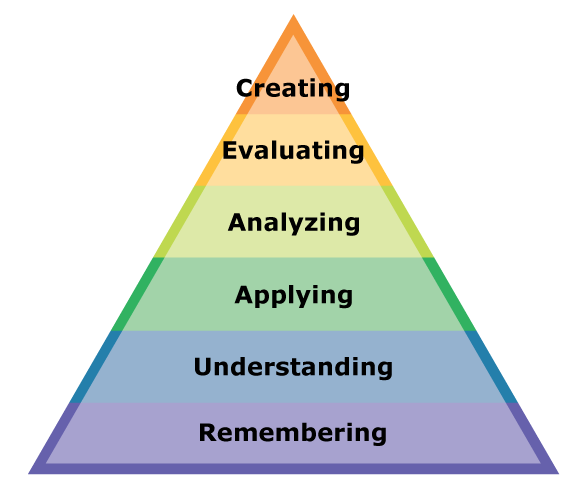
\includegraphics[width=4cm]{Bloom's Pyramid.png}}
        \caption{Knowledge Levels of Bloom's Pyramid}
        \centering{\label{fig}}
    \end{figure}
\end{center}

We figured that following this steps would be the best way to start our project so the first stage was to remember the theory given in the course classes and we even checked all the course subjects that we considered important to the realization of the project. The next steps were to understand everything that was being given to us (initial code, utterance, tests, report format, etc) and starting to apply what was necessary for the parallelization of the program. The next two phases (analyzing and evaluating) were done simultaneously, as we started taking note of the responses from our parallel program as soon as we started testing our solution. The last stage of the pyramid was implemented after realizing what were the pros and cons of our parallel solution and figuring out if it was necessary to change something in our program in order to get a better solution.

%\hfill June 06, 2021

\section{Beforehand concepts}
We're gonna explain some concepts before going further. These are for analysis and evaluation purposes.

\subsection{Class contents}
\begin{itemize}
    \item \textbf{Speedup} is given by the ratio of the time it takes the sequential version to execute for the time it takes the parallel version to execute.
    \item \textbf{Efficiency} is given by the ratio of the Speedup for the number of threads that ran during the parallel program.
    \item \textbf{Cost} is given by the time of the parallel execution times the number of threads that ran during it's execution.
    \item \textbf{Amdahl's Law} gives us an upper bound for the speedup, assuming that we want to compute the same work as in the sequential version. This assumption is correct because increasing the work won't help us in this project, our goal is to decrease the time it takes to compute the \underline{same amount of work}.
\end{itemize}

\subsection{Concept application in this project}
The speedup is an obvious choice for measuring how faster our parallel version is than the sequential. Efficiency and cost are used for checking if our solution is optimal. \textbf{Amdahl's Law isn't applied directly. It's more of a curiosity after getting our results to define an upper bound for the speedup and compute the sequential fraction of the algorithm.}
\begin{center}
\textit{\\"A parallel algorithm is cost-optimal if\\ Efficiency = 100\% and Cost = Sequential Time"}
\end{center}

\section{Analysis and approach} \label{analysisandapproach}

\subsection{Code analysis}

The sequential base of this project presented a few situations where concurrency could be used to our advantage. The initialization of the layer and layer\_copy arrays was being made with the usage of two identical loops, so we found that merging those "for's" was helpful to later parallelize their computation with the use of OpenMP. Going further, we found at the "4.2" area of the code a similar loop to the one above it, so we decided to create an if statement that would only set values on the layer\_copy array when the final storm had finished updating the energy values of the layer array allowing us to merge another for and later utilize OpenMP. On the "4.3" we found an area of code where a maximum was being maintained over a sequential loop, so we marked it as a possible critical area of our code when attempting to parallelize that same "for". Finally we also found that the layer and layer\_copy were not being freed at the end of the program, so we did that just for consistency sake, even though it is not really the purpose of this class.

\subsection{Approach to OpenMP solution}

When trying to introduce OpenMP to our sequential code, we had a few difficulties trying to find a solution that both maintained the correct results and had a decent speedup performance wise.
\begin{itemize}
    \item We tried to collapse as many nested loops as possible, but dealing with the incoming dependencies proved to be too much too handle on some occasions. For example the "4.1" area of the code seemed a good spot to introduce the collapse statement on the nested for loops handling the "j" and "k" variables, but we were not able to decompose the dependencies brought by the energy and position variables, and so we ended up only parallelizing the "k" for loop, and merging the "4.2.1" loop into it, since they had the same number of iterations and their dependencies only required a single if statement to be introduced.
    \item After the issue mentioned above, our biggest barrier to parallelization was definetely the "4.3" code area. Our first approach was to collapse the loop above on the "4.2.2" area with it, since they had the same number of iterations and iterated through the same variable values. We attempted to fill layer[1] with its correct value before the loop, sequentially, and then inside the loop to find calculate the value of layer[k] before going through the nested if statements and the maximum update, but this only created extra dependencies that we could not solve, so we ended up running the for loops separately but concurrently, and of course we created a critical zone where the maximum was being updated, so the results were kept consistent with the sequential version
\end{itemize}

\section{Testing and correcting}
Regarding the testing phase, we started testing our code as soon as we knew it would run correctly. As told in the introduction, analysis and evaluation were done simultaneously, so we wanted to test extensively our code. Unfortunately, this didn't go according to our expectations because of the time limit, however we managed to test our code enough so we could get good results and take good conclusions out of them.
\\
For testing purposes we started by making a python script that would run both sequential and parallel versions of the algorithm for each each test (or accumulations of tests). The script would check if both outputs (using debug mode) were the same, and if so, it would return the speedup. We spent a good amount of time using that script for testing - and we managed to encounter some errors during that time which we, obviously, corrected. However, a script like this wasn't enough so later we started using some scripts a colleague of ours made and posted on piazza. As we ran out of time we chose to use them (later giving them credit of course) instead of making our own. With these scripts we managed to compare results much faster and generate plots which make analysis easier.

\subsection{Final solution}
Having in mind the previous analysis, we decided to change some of the code the code in a way we could control the number of threads. By changing that we could see effectively (with help of the scripts) which were the numbers of threads that were most effective for our solution. Of course we kept in mind that that number is result of the machine we're running the code in, so we wanted to test our code in a machine capable of running more threads in the cluster - we couldn't reserve a node with more threads than the machine we were running the code in (twelve threads max) so we opted for not testing our code in the cluster as we don't think it'll get us anywhere.

Unfortunately though, we ran out of time before we could try to evaluate and parallelize other sections of the code beyond section 4. This was not our expectations for this project at all, but given the situation we decided to work with this solution until the end.

\section{Results}
When we reached our final solution we started testing it extensively. Our main focus was to use different amounts of threads and then compare the results as plotted graphs. We also tried to create different tests where a wide array of layer and storm sizes was tested so we were able to analyse the performance of our code with a good degree of certainty. In the end we had divided those tests into three experiments. The first two tested a wide array of storms on a large layer, with the intent of testing most aspects of our solution and the code base. The third one consisted of a extremely large storm of points to try and find an extreme barrier to our solution's performance. In the end our results were plotted into graphs, so we could more easily distinguish increases and decreases of performance, we also included the results from the sequential version so we could understand how our solution compared with the code base that was given to us at the beginning of the project. 

\subsection{Performance}
From the results of our testing we wanna highlight a few cases that we feel illustrate the performance of our program the best. Keep in mind these tests were also done twice for consistency sake.

\begin{center} \label{fig2}
    \begin{figure}[htbp]
        \centering{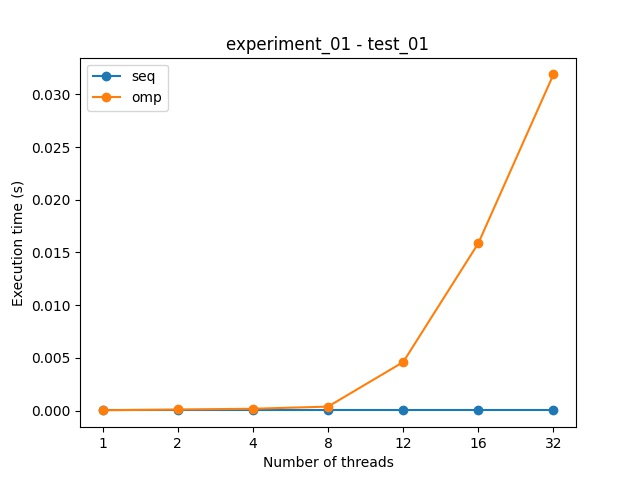
\includegraphics[width=6cm]{test_01.jpg}}
        \caption{Test 1 plotted graph}
        \centering{\label{fig}}
    \end{figure}
\end{center}

On this first test we are using a small layer and small storms, and we see immediate results of this situation. The overhead of the many operations called by the concurrent implementation like thread creation and management quickly overpower the small computational needs of the problem, meaning we end up with worse results than just running our code sequentially.

\begin{center} \label{fig3}
    \begin{figure}[htbp]
        \centering{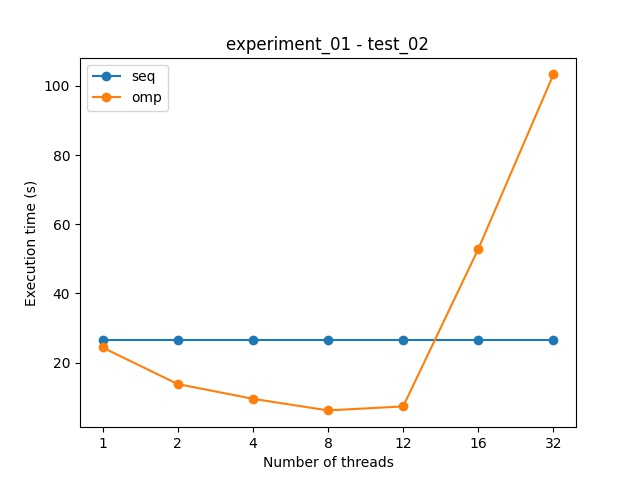
\includegraphics[width=6cm]{test_02.jpg}}
        \caption{Test 2 plotted graph}
        \centering{\label{fig}}
    \end{figure}
\end{center}

On this second test we went for a bigger layer, with a size of thirty thousand, and twenty thousand points in each storm, so we can finally see our usage of threads get some performance increase from the sequential version. Where the base version maintained its constant results, we were able to notice a performance increase until eight to twelve threads were being used, and above that our performance dipped immensely, with our computation times skyrocketing past the sequential version.

\begin{center} \label{fig4}
    \begin{figure}[htbp]
        \centering{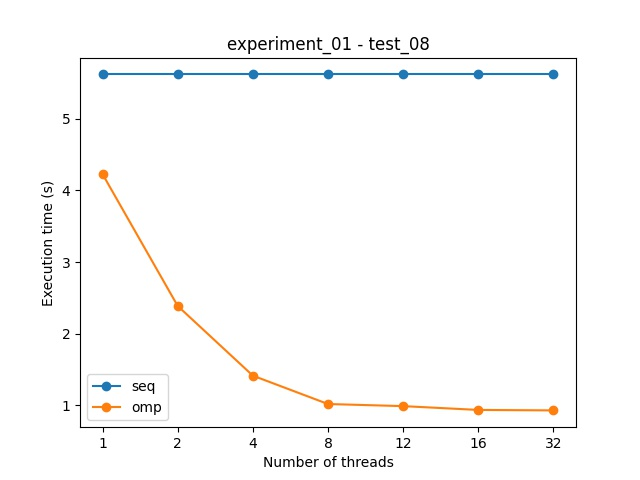
\includegraphics[width=6cm]{test_08.jpg}}
        \caption{Test 8 plotted graph}
        \centering{\label{fig}}
    \end{figure}
\end{center}

On this test we decided to find a limit to our layer initialization concurrency, so we created a one hundred million slot array with only a single storm (which had only one hit of a particle). This proved to be pretty successful, as we were able to notice performance increases from two to thirty-two threads.

%mudar se o teste do madeira chegar a acabar antes
\begin{center} \label{fig5}
    \begin{figure}[htbp]
        \centering{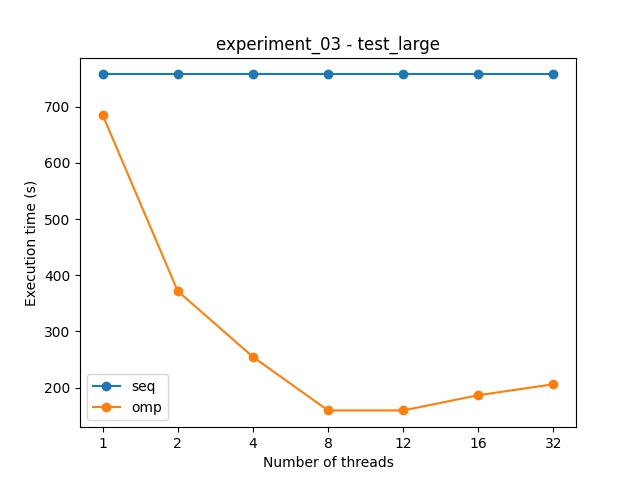
\includegraphics[width=6cm]{test_large.jpg}}
        \caption{Custom test plotted graph}
        \centering{\label{fig}}
    \end{figure}
\end{center}

On our final test we also went for the approach of finding a limit, but this time by overloading a single storm with one hundred thousand hits, on a layer of size equal to one million. This result in conjunction with the one pictured in Fig.3 showed the weaknesses of our solution, as we did not apply concurrency to the computing of the energy and position of each hit, so both hit heavy tests saw big performance dips, as a final statement in regard to our solution's performance, we think this area is where the biggest amount of improvement can come, if more time and attention was given to dealing with the dependencies that appear with the merging of both for loops on the "4.1" area of the code.

\subsubsection{Performance measurement}
We talked about some class concepts in the beginning of the report but we have yet to use them as we didn't until now.
\begin{itemize}
    \item For \ref{fig2} the speedup is optimal when only one thread is used. As the number of threads are increased speedup decreases more and more. As a result of this, the efficiency of the solution is also decreasing. The cost of the algorithm, as thread number increase becomes huge.
    \item For \ref{fig3} we have our optimal speedup at eight threads. Until eight threads the time is decreasing, however the efficiency is decreasing and cost is increasing.
    \item For \ref{fig4} the optimal speedup is at thirty-two threads. We can notice the efficiency is also decreasing in this case and the cost is increasing.
    \item For \ref{fig5} the speedup is increasing until eight threads. Once again efficiency is decreasing and cost is increasing as number of threads increases
\end{itemize}

Given this, from the cases where the parallel version is faster, we can observe that the times where \textbf{efficiency is greater is when we're using only two threads}. We can also notice that the \textbf{time of execution is fastest when using eight threads}. Calculating the average of the optimal speedups we get a number close to 5. We haven't made so many tests it would be obvious to know what the maximum speedup could be. However we could apply Amdahl's law in reverse. If we assume speedup is at max 5, then we can assume that the sequential part of this algorithm is at least 


\section{Conclusion}
Initially, our focus was to understand the reason for parallelism of program instructions and, as we were analyzing and evaluating our solutions, we began to realize that the success of parallelism is not only related to program optimization but it also has to do with the type and the size of the problem, as well as the environment in which we ran it. In certain cases, the existence of parallelism allows us to obtain a much higher efficiency than a sequential version of the program. In other cases, from a certain number of threads, the sequential program surpasses the efficiency of the parallel program, since the creation of threads has an inherent cost to the application when running tests. Thus, in this situation, these costs make, the parallel program heavier than the sequential.\\
We've also learned that it's very important to find a good solution to the problem, but beyond that, it's also very important to test our solution extensively. This was very beneficial for us because it made us understand a lot more about OpenMP's functionalities, know how to analyze and evaluate our program in order to be able to correct parallelism problems or even optimize these solutions, and putting these last points together, understand all the strengths and weaknesses of our program.



% use section* for acknowledgment
\ifCLASSOPTIONcompsoc
  % The Computer Society usually uses the plural form
  \section*{Acknowledgments}
\else
  % regular IEEE prefers the singular form
  \section*{Acknowledgment}
\fi


We would like to thank:
\begin{itemize}
    \item Everyone that helped us indirectly through Piazza workspace, namely on threads @77 (João Antão and his colleagues from Group 15, Jorge Coelho)...
    \item Group 40 which helped us repairing some errors we had in our code 
\end{itemize}

% Can use something like this to put references on a page
% by themselves when using endfloat and the captionsoff option.
\ifCLASSOPTIONcaptionsoff
  \newpage
\fi


\begin{thebibliography}{1}

\bibitem{surveyTools}
Mubrak S. Mohsen, Rosni Abdullah, and Yong M. Teo, \emph{A Survey on Performance Tools for OpenMP}, 2009, p.1

\end{thebibliography}

% that's all folks
\end{document}